\documentclass[letterpaper,11pt]{article}

\usepackage{amsmath}
\usepackage{amssymb}
\usepackage{bm}
\usepackage[hmargin=1.25in,vmargin=1in]{geometry}
\usepackage{booktabs}
\usepackage{graphicx}
\usepackage{hyperref}
\usepackage{lmodern}
\usepackage{microtype}
\usepackage{subcaption}

\title{Final: STAT 570}
\author{Philip Pham}
\date{\today}

\begin{document}
\maketitle

Consider the failure time data in Table \ref{tab:failure_time_data}.

\begin{enumerate}
\item We describe a simple model for these data. Let $p$ ($0 < p < 1$) denote
  the weekly failure probability, i.e., the probability of failure during any
  week, and $T$ the random variable describing the week at which failure
  occurred. Then $T$ may be modeled as a geometric random variable:
  \begin{equation}
    \mathbb{P}\left(T = t \mid p\right)
    = \begin{cases}
      p\left(1-p\right)^{t-1}, &t=1,2,\ldots; \\
      0,&\text{otherwise}.      
    \end{cases}
    \label{eqn:p1_model}
  \end{equation}

  Let $Y_t$ represent the number of components that fail in week $t$,
  $t = 1,2,\ldots,N$, and $Y_{N+1}$ the number of components that have not failed
  by week $N$.

  \begin{enumerate}
  \item Show that the likelihood function is
    \begin{equation}
      L\left(p\right) =
      \left[\left(1 - p\right)^N\right]^{Y_{N+1}}
      \prod_{t=1}^N\left[
        p\left(1 - p\right)^{t-1}
      \right]^{Y_t}.
      \label{eqn:p1_likelihood}
    \end{equation}
    \begin{description}
    \item[Solution:] An individual component's failure week has distribution
      $\operatorname{Geometric}\left(p\right)$. The probability that a single
      component fails in week $t$ is the probability that it survived $t - 1$
      weeks and failed on week $t$, which is $p\left(1 - p\right)^{t-1}$ from
      Equation \ref{eqn:p1_model}. There are $Y_t$ such components, which gives
      us the factors for $t = 1,2,\ldots,N$.

      The probability that a component fails at a later date is
      \[
        \left(1 - p\right)^N\sum_{k=1}^\infty p\left(1-p\right)^{k-1}
        =
        \left(1 - p\right)^N\frac{p}{1 - \left(1 - p\right)}
        =
        \left(1 - p\right)^N,
      \]
      which gives us the remaining factor. There are $Y_{N+1}$ remaining
      components, so
      \[
        L\left(p\right) =
        \left\{
          \prod_{t=1}^N \left[
            p\left(1 - p \right)^{t-1}
          \right]^{Y_t}
        \right\}
        \times
        \left[\left(1-p\right)^N\right]^{Y_{N+1}}.
      \]
    \end{description}
  \item Find an expression for the MLE $\hat{p}$.
    \begin{description}
    \item[Solution:] 
      The score function is
      \begin{align}
        S\left(p\right)
        &= \frac{\partial}{\partial p}\log L\left(p\right) \nonumber\\
        &= \frac{\partial}{\partial p}\left[
          NY_{N + 1}\log\left(1 - p\right)
          + \sum_{t=1}^N Y_t\left(
          \log p + \left(t - 1\right)
          \log\left(1 - p\right)
          \right)
          \right]\nonumber\\
        &= -\frac{NY_{N+1}}{1 - p}
          + \sum_{t=1}^N Y_t\left(
          \frac{1}{p}
          -
          \frac{t - 1}{1 - p}
          \right)
        = -\frac{NY_{N+1}}{1 - p}
          + \sum_{t=1}^N Y_t
          \frac{1-pt}{p\left(1 - p\right)}.
          \label{eqn:p1_score}
      \end{align}

      Solving for $S\left(\hat{p}\right) = 0$, we find the MLE:
      \begin{equation}
        \hat{p}\left(
          NY_{N+1} + \sum_{t=1}^{N}tY_t
        \right) = \sum_{t=1}^N Y_t
        \implies
        \boxed{
          \hat{p} = \frac{\sum_{t=1}^N Y_t}
          {NY_{N+1} + \sum_{t=1}^{N}tY_t}.
        }
        \label{eqn:p1_mle}
      \end{equation}
    \end{description}
  \item Find the form of the observed information and hence the asymptotic
    variance of the maximum likelihood estimate (MLE).
    \begin{description}
    \item[Solution:] Using Equation \ref{eqn:p1_score}, the expected observed
      information is
      \begin{align}
        I\left(p\right)
        &= \mathbb{E}\left[-\frac{\partial}{\partial p}S\left(p\right) \mid p\right]
          \nonumber\\
        &= \frac{N\mathbb{E}\left[Y_{N+1} \mid p\right]}{(1-p)^2}
          + \sum_{t=1}^N\mathbb{E}\left[Y_t \mid p\right]
          \left(
          \frac{1}{p^2} + \frac{t-1}{\left(1-p\right)^2}
          \right)
          \nonumber \\
        &= n\frac{N\left(1-p\right)^N}{(1-p)^2}
          + np\sum_{t=1}^N
          \left(1 - p\right)^{t-1}
          \left(
          \frac{1}{p^2} + \frac{t-1}{\left(1-p\right)^2}
          \right)
          \nonumber \\
        &= n\left[
          \frac{\left(1-p\right)^N}{(1-p)^2}
          +
          \frac{1 - \left(1 - p\right)^N}{p^2}
          +
          \frac{(1-p) - (1-p)^N}{p(1-p)^2}
          \right] \nonumber \\
        &= \boxed{n\frac{1 - \left(1 - p\right)^N}
          {p^2\left(1 - p\right)},} \label{eqn:p1_fisher_information}
      \end{align}
      where $n = Y_{N+1} + \sum_{t=1}^N Y_t$.

      From Equation \ref{eqn:p1_fisher_information}, the asymptotic variance of
      $\hat{p}$ is
      \begin{equation}
        \operatorname{var}\left(\hat{p}\right)
        \approx
        \hat{\operatorname{var}}\left(\hat{p}\right) = 
        I\left(\hat{p}\right)^{-1} = \frac{1}{n} \times
        \frac{\hat{p}^2\left(1-\hat{p}\right)}
        {1 - \left(1-\hat{p}\right)^N}
        \label{eqn:p1_variance}
      \end{equation}
      by asymptotic normality of the MLE.
    \end{description}
  \item For the data in Table \ref{tab:failure_time_data}, calculate the MLE,
    $\hat{p}$. the variance of $\hat{p}$, and an asymptotic
    95\% confidence interval for $p$.

    \begin{description}
    \item[Solution:] The MLE can be calculated with Equation \ref{eqn:p1_mle} to
      be $\boxed{\hat{p} = 0.354717.}$ The variance can be found with Equation
      \ref{eqn:p1_variance} to be
      $\boxed{\hat{\operatorname{var}}\left(\hat{p}\right) = 0.00016828.}$

      If $\Phi$ is the cumulative distribution function for a standard normal,
      we can use asymptotic normality to find the 95\% confidence interval as
      \begin{equation*}
        \left[
          \hat{p} +
          \Phi^{-1}\left(0.025\right)\sqrt{\hat{\operatorname{var}}\left(\hat{p}\right)},
          \hat{p} +
          \Phi^{-1}\left(0.975\right)\sqrt{\hat{\operatorname{var}}\left(\hat{p}\right)}
        \right]
        =
        \boxed{\left[0.32929,0.38014\right].}
      \end{equation*}
    \end{description}
  \item We now consider a Bayesian analysis. The conjugate prior for $p$ is a
    beta distribution, $\operatorname{Beta}\left(a, b\right)$. State the form of
    the posterior with this choice. Give the form of the posterior mean and
    write as a weighted combination of the MLE and the prior mean.

    \begin{description}
    \item[Solution:] By Bayes' rule, we know the posterior density is
      proportional to the likelihood times the prior. From Equation
      \ref{eqn:p1_likelihood}, we'll have
      \begin{align*}
        L\left(p\right) \times \left[
        p^{a-1}\left(1-p\right)^{b-1}
        \right]
        &= p^{a-1}\left(1 - p\right)^{b + NY_{N+1} - 1}
          \prod_{t=1}^N\left[
          p\left(1 - p\right)^{t-1}
          \right]^{Y_t} \\
        &= p^{a + \sum_{t=1}^N Y_t -1}
          \left(1 - p\right)^{b + \sum_{t=1}^N (t-1)Y_t + NY_{N+1} - 1},
      \end{align*}
      whose form we recognize as the integrand of beta function, so the
      posterior also has beta distribution, that is,
      \begin{align}
        p \mid Y_1,Y_2,\ldots,Y_{N+1}
        &\sim \operatorname{Beta}\left(
          a + \sum_{t=1}^N Y_t,
          b + \sum_{t=1}^N (t-1)Y_t + NY_{N+1}
          \right) \nonumber\\
        &= \frac{\Gamma\left(a^\prime + b^\prime\right)}
          {\Gamma\left(a^\prime\right)\Gamma\left(b^\prime\right)}
          p^{a^\prime -1}\left(1 - p\right)^{b^\prime - 1},
          \label{eqn:p1_posterior}
      \end{align}
      where $a^\prime = a + \sum_{t=1}^N Y_t$ and
      $b^\prime = b + \sum_{t=1}^N (t-1)Y_t + NY_{N+1}$.

      The posterior mean takes the form
      \begin{align}
        \mathbb{E}\left[
        p \mid Y_1,Y_2,\ldots,Y_{N+1}
        \right]
        &= \frac{a^\prime}{a^\prime + b^\prime}
          \nonumber \\
        &= \frac{a + \sum_{t=1}^N Y_t}
          {a + b + \sum_{t=1}^N tY_t + NY_{N+1}}. \label{eqn:p1_posterior_mean}
      \end{align}

      We have that the prior mean is $p_{\mathrm{prior}} = \frac{a}{a + b}$.
      Equation \ref{eqn:p1_posterior_mean} can be rewritten as
      \begin{equation}
        \boxed{
        \frac{
          \left(a + b\right)
          p_{\mathrm{prior}}
          +
          \left(
            \sum_{t=}^N tY_t + NY_{N+1}
          \right)
          \hat{p}}
          {a + b + \sum_{t=}^N tY_t + NY_{N+1}},}
        \label{eqn:p1_posterior_mean_sum}
      \end{equation}
      so the posterior mean is a convex combination of the prior mean and MLE.
    \end{description}
  \item Suppose we wish to fix the parameters of the prior, $a$ and $b$, so that
    the mean is $\mu$ and the prior standard deviation is $\sigma$. Obtain
    expressions for $a$ and $b$ in terms of $\mu$ and $\sigma^2$.
    \begin{description}
    \item[Solution:] It is well known that the mean and variance of the
      $\operatorname{Beta}\left(a,b\right)$ distribution are $\frac{a}{a+b}$ and
      $\frac{ab}{(a+b)^2(a+b+1)}$, respectively.

      Solving equations
      \begin{align*}
        \frac{a}{a + b}
        &= \mu \\
        \frac{ab}{(a+b)^2(a+b+1)} &= \sigma^2,
      \end{align*}
      we find that
      \begin{align}
        a
        &= \mu\left[
          \frac{\mu\left(1 - \mu\right)}{\sigma^2} - 1
          \right]
          \label{eqn:p1_a} \\
        b
        &=  \left(1 - \mu\right)\left[
          \frac{\mu\left(1 - \mu\right)}{\sigma^2} - 1
          \right].
          \label{eqn:p1_b}
      \end{align}
    \end{description}
  \item For the data in Table \ref{tab:failure_time_data}, assume we wish to
    have a beta prior with $\mu = 0.2$ and $\sigma = 0.08$. State the posterior
    for the prior corresponding to this choice and evaluate the posterior
    mean. Simulate samples from the posterior distribution. Provide a histogram
    representation of the posterior distribution and calculate the 5\%, 50\% and
    95\% points of the posterior distribution.

    \begin{figure}
      \centering
      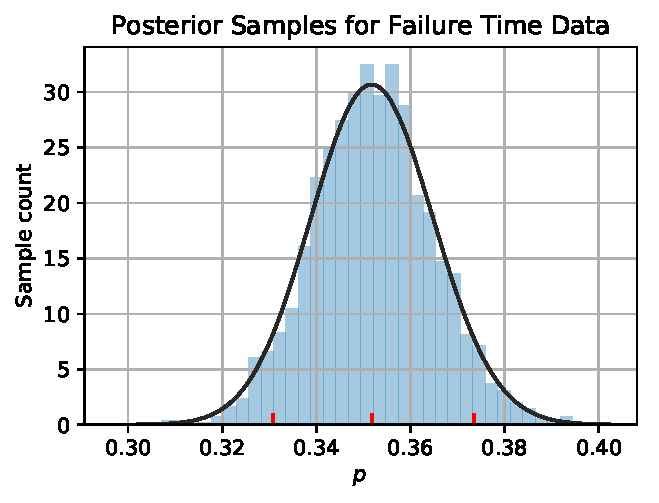
\includegraphics{p1_posterior_samples.pdf}
      \caption{2,048 samples drawn from the posterior in Equation
        \ref{eqn:p1_posterior_data}. The red ticks denote the 5\%, 50\% and
        95\% quantiles.}
      \label{fig:p1_posterior_samples}
    \end{figure}
    
    \begin{description}
    \item[Solution:] Apply Equations \ref{eqn:p1_a} and \ref{eqn:p1_b} with
      $\mu = 0.2$ and $\sigma = 0.08$, we find the prior:
      \begin{equation}
        p \sim \operatorname{Beta}\left(4.8, 19.2\right).
        \label{eqn:p1_prior}
      \end{equation}

      Using Equation \ref{eqn:p1_posterior}, we have find the posterior:
      \begin{equation}
        p \sim \operatorname{Beta}\left(474.8, 874.2\right).
        \label{eqn:p1_posterior_data}
      \end{equation}
      
      A histogram of samples drawn from the distribution in Equation
      \ref{eqn:p1_posterior_data} can be found in Figure
      \ref{fig:p1_posterior_samples}. The 5\%, 50\%, and 95\% posterior
      quantiles are 0.33070873, 0.35189124, and 0.37346975, respectively.

      Code for the histogram can be found in
      \href{http://nbviewer.jupyter.org/github/ppham27/stat570/blob/master/final/failure\_time.ipynb}{\texttt{failure\_time.ipynb}}.
    \end{description}
  \end{enumerate}
\item
  \begin{enumerate}
  \item A more complex likelihood for these data would assume that the $i$-th
    component had their own probability $p_i$, with the $p_i$'s arising from a
    distribution $\pi\left(p\right)$. Show that
      \begin{equation}
        \mathbb{P}\left(T = t\right) =
        \mathbb{E}\left[(1 - p)^{t-1}\right] -
        E[(1 - p)^t],
        \label{eqn:p2_pmf}
      \end{equation}
      and
      \begin{equation}
        \mathbb{P}\left(T > t\right) = \mathbb{E}\left[(1 - p)^t\right].
        \label{eqn:p2_survival}
      \end{equation}
      \begin{description}
      \item[Solution:] First let us find the survival function in
        \ref{eqn:p2_survival}.
        \begin{align*}
          \mathbb{P}\left(T > t\right)
          &= \int_0^1
          \mathbb{P}\left(T > t \mid p\right)
          \pi\left(p\right)\,\mathrm{d}p 
          = \int_0^1 \left[\sum_{s=t + 1}^\infty p(1 - p)^{s-1}\right]
            \pi\left(p\right)
          \,\mathrm{d}p \\
          &= \int_0^1 \left[p\sum_{s=0}^\infty (1 - p)^s\right]
            (1 - p)^t
            \pi\left(p\right)
            \,\mathrm{d}p \\
          &= \int_0^1 \left[p \times \frac{1}{1 - (1-p)}\right]
            (1 - p)^t
            \pi\left(p\right)
            \,\mathrm{d}p
          = \int_0^1 (1 - p)^t
            \pi\left(p\right)
            \,\mathrm{d}p \\
          &= \mathbb{E}\left[\left(1-p\right)^t\right],
        \end{align*}
        which proves Equation \ref{eqn:p2_survival}.

        The probability mass function in Equation \ref{eqn:p2_pmf} follows:
        \begin{equation*}
          \mathbb{P}\left(T = t\right)
          = \mathbb{P}\left(T > t - 1\right)
          - \mathbb{P}\left(T > t\right)
          = \mathbb{E}\left[\left(1-p\right)^{t-1}\right]
          - \mathbb{E}\left[\left(1-p\right)^{t}\right].
        \end{equation*}
      \end{description}
    \item Obtain expressions for
      $\mathbb{P}\left(T = t \mid \alpha, \beta\right)$ and
      $\mathbb{P}\left(T > t \mid \alpha, \beta\right)$ with
      $\pi\left(\cdot\right)$ taken as the beta distribution,
      $\operatorname{Beta}\left(\alpha, \beta\right)$.

      \begin{description}
      \item[Solution:] These follow from Equations
        \ref{eqn:p2_pmf} and \ref{eqn:p2_survival}.

        \begin{align}
          \mathbb{P}\left(T > t\right)          
          &= \mathbb{E}\left[
            (1 - p)^t
            \right]
            = \sum_{s=t}^\infty
            \mathbb{E}\left[
            p\left(1 - p\right)^s
            \right] \label{eqn:p2_survival_beta}\\
          &=
            \sum_{s=t}^\infty
            \int_0^p
            p\left(1-p\right)^s
            \frac{\Gamma\left(\alpha + \beta\right)}            
            {\Gamma\left(\alpha\right)\Gamma\left(\beta\right)}
            p^{\alpha - 1}\left(1-p\right)^{\beta-1}
            \,\mathrm{d}p
          \nonumber\\
          &= \sum_{s=t}^\infty
            \int_0^p
            \frac{\Gamma\left(\alpha + \beta\right)}
            {\Gamma\left(\alpha\right)\Gamma\left(\beta\right)}
            p^{\alpha + 1 - 1}\left(1-p\right)^{\beta + s -1}
            \,\mathrm{d}p \nonumber\\
          &= \frac{\Gamma\left(\alpha + \beta\right)} 
            {\Gamma\left(\alpha\right)\Gamma\left(\beta\right)}            
            \sum_{s=t}^\infty
            \frac
            {\Gamma\left(\alpha + 1\right)\Gamma\left(\beta + s\right)}
            {\Gamma\left(\alpha + \beta + s + 1\right)}
            = \alpha\frac{\Gamma\left(\alpha + \beta\right)} 
            {\Gamma\left(\beta\right)}
            \sum_{s=t}^\infty
            \frac
            {\Gamma\left(\beta + s\right)}
            {\Gamma\left(\alpha + \beta + s + 1\right)}
          \nonumber\\
          &= 
            1
            - \alpha
            \frac{\Gamma\left(\alpha + \beta\right)} 
            {\Gamma\left(\beta\right)}
            \sum_{s=0}^{t-1}
            \frac
            {\Gamma\left(\beta + s\right)}
            {\Gamma\left(\alpha + \beta + s + 1\right)} \nonumber\\
          &= 1 - \frac{1}{B\left(\alpha,\beta\right)}
            \sum_{s=0}^{t-1} B\left(\alpha + 1, \beta + s\right)
            = \frac{B\left(\alpha,\beta + t\right)}{B\left(\alpha,\beta\right)}
            = \frac{\Gamma\left(\alpha + \beta\right)\Gamma\left(\beta + t\right)}
            {\Gamma\left(\beta\right)\Gamma\left(\alpha + \beta + t\right)}
            \nonumber
        \end{align}
        where $B$ is the beta function, and we know
        $\mathbb{P}\left(T > 0\right) = 1$.

        Plugging Equation \ref{eqn:p2_survival_beta} into Equation
        \ref{eqn:p2_pmf}, one obtains
        \begin{equation}
          \mathbb{P}\left(T = t\right)
          = \frac{B\left(\alpha + 1, \beta + t - 1\right)}{B\left(\alpha,\beta\right)}
          = \alpha
          \frac{\Gamma\left(\alpha + \beta\right)\Gamma\left(\beta + t - 1\right)}
          {\Gamma\left(\beta\right)\Gamma\left(\alpha + \beta + t\right)}
          \label{eqn:p2_pmf_beta}
        \end{equation}
        for $t \in \mathbb{N}$.
      \end{description}
    \item Using the previous part, write down the likelihood function
      $L\left(\alpha, \beta\right)$ corresponding to data
      $\left\{Y_t\right\}_{t=1}^{N+1}$.

      \begin{description}
      \item[Solution:] Our model for $T$ is different, so we can substitute
        Equations \ref{eqn:p2_pmf_beta} and \ref{eqn:p2_survival_beta} into
        Equation \ref{eqn:p1_likelihood}: we'll have
        $\mathbb{P}\left(T = t\right)$ in place of $p\left(1 - p\right)^{t-1}$
        and $\mathbb{P}\left(T > N\right)$ in place of $\left(1 - p\right)^N$.
        \begin{align}
          L\left(\alpha,\beta\right)
          &= \left[\mathbb{P}\left(T > N\right)\right]^{Y_{N+1}}
            \prod_{t=1}^N\left[\mathbb{P}\left(T = t\right)\right]^{Y_t}
            \label{eqn:p2_likelihood} \\
          &= \left[
            \frac{B\left(\alpha, \beta + N\right)}{B\left(\alpha, \beta\right)}
            \right]^{Y_{N+1}}
            \prod_{t=1}^N \left[
            \frac{B\left(\alpha + 1, \beta + t - 1\right)}
            {B\left(\alpha, \beta\right)}
            \right]^{Y_t}.
            \nonumber
        \end{align}
      \end{description}
    \item Find the MLEs  $\hat\alpha$ and $\hat\beta$ for the data of Table
      \ref{tab:failure_time_data}.
      \begin{description}
      \item[Solution:] From Equation \ref{eqn:p2_likelihood}, we can consider
        the log-likelihood function:
        \begin{align}
          &l\left(\alpha,\beta\right)
          =
          \log L\left(\alpha,\beta\right)
          \label{eqn:p2_log_likelihood} \\
          &= -n\log B\left(\alpha,\beta\right)
            +
            Y_{N+1}\log B\left(\alpha,\beta+N\right)
            +
            \sum_{t=1}^N Y_t\log 
            B\left(\alpha + 1, \beta + t - 1 \right).
            \nonumber
        \end{align}

        The score function is
        \begin{align}
          S\left(\alpha,\beta\right) &= 
          \nabla l\left(\alpha,\beta\right)
          = \begin{pmatrix}
            S_\alpha\left(\alpha,\beta\right) \\
            S_\beta\left(\alpha,\beta\right)
          \end{pmatrix} \label{eqn:p2_score}\\
          S_\alpha\left(\alpha,\beta\right)
          &= -n\left[
            \psi\left(\alpha\right) -
            \psi\left(\alpha + \beta\right)
            \right]
            + Y_{N+1}\left[
            \psi\left(\alpha\right)-
            \psi\left(\alpha + \beta + N\right)              
            \right] \nonumber\\
          &~~~~~+ \sum_{t=1}^N Y_{t}\left[
            \psi\left(\alpha + 1\right) -
            \psi\left(\alpha + \beta + t\right)            
            \right],
            \nonumber \\
          S_\beta\left(\alpha,\beta\right)
          &= -n\left[
            \psi\left(\beta\right) -
            \psi\left(\alpha + \beta\right)
            \right]
            + Y_{N+1}\left[
            \psi\left(\beta + N\right)-
            \psi\left(\alpha + \beta + N\right)              
            \right] \nonumber\\
          &~~~~~+ \sum_{t=1}^N Y_{t}\left[
            \psi\left(\beta + t - 1\right) -
            \psi\left(\alpha + \beta + t\right)            
            \right], \nonumber
        \end{align}p
        where
        $\psi\left(x\right) = \Gamma^\prime\left(x\right)/\Gamma\left(x\right)$
        is the digamma function.

        Numerically solving Equation \ref{eqn:p2_score} for
        $S\left(\hat\alpha,\hat\beta\right) = \mathbf{0}$, I obtain
        $\boxed{\hat\alpha = 1.413336}$ and $\boxed{\hat\beta = 1.38001102}$
        for the MLEs.
      \end{description}
    \end{enumerate}
  \item \begin{enumerate}
    \item Show that the likelihood in Equation \ref{eqn:p1_likelihood} can be
      written as a product of binomial distributions.

      \begin{description}
      \item[Solution:] We can model the data as taking $N$ draws from a binomial
        distribution. Following each draw, we discard the failures and make
        another draw if $t < N$:
        \begin{align}
          L\left(p\right)
          &= \prod_{t=1}^N \left[
            {n - \sum_{s=1}^{t-1}Y_s
            \choose Y_t}p^{Y_t}\left(1 - p\right)^{n - \sum_{s=1}^{t}Y_s}
            \right]
            \label{eqn:p3_likelihood} \\
          &= \prod_{t=1}^N \left[
            {\sum_{s = t}^{N+1}Y_s \choose Y_t}
            p^{Y_t}\left(1 - p\right)^{\sum_{s = t + 1}^{N+1} Y_s}\right],
            \nonumber
        \end{align}
        which is equivlaent to Equation \ref{eqn:p1_likelihood} up to a constant
        of proportionality,

        In Equation \ref{eqn:p3_likelihood}, we have a product of binomial
        probability mass functions, where
        $Y_t \mid Y_1,\ldots,Y_{t-1} \sim \operatorname{Binomial}\left(
          n - \sum_{s=1}^{t - 1}Y_s, p \right).$
      \end{description}
    \item Fit the binomial model, and show that the estimate of the probability
      is identical to that under the previous MLE analysis. Obtain a 95\%
      asymptotic confidence interval for $p$.
      \begin{description}
      \item[Solution:] Since Equation \ref{eqn:p3_likelihood} only differs from
        Equation \ref{eqn:p1_likelihood} by a constant of proporitionality, the
        score function is also Equation \ref{eqn:p1_score}. Thus, the MLE is
        same $\hat{p} = 0.354717$.

        The observed information will also be the same. To calculate the
        expected observed information, we can use the law of total expectation
        and strong induction. For the base case
        $\mathbb{E}\left[Y_1\right] = np$. In general,
        $\mathbb{E}\left[Y_t\right] = np\left(1 - p\right)^{t-1}$ for
        $t = 1,2,\ldots,N$. For $t > 1$, we have
        \begin{align}
          \mathbb{E}\left[Y_t\right]
          &=  
            \mathbb{E}\left[\mathbb{E}\left[Y_t \mid Y_1,\ldots,Y_{t-1}\right]\right]
          =
            \mathbb{E}\left[
            p\left(n - \sum_{s=1}^{t-1}Y_s\right)
            \right] \nonumber\\
          &= p\left(n - \sum_{s=1}^{t-1}\mathbb{E}\left[Y_s\right]\right)
          =
            p\left(n - \sum_{s=1}^{t-1} np\left(1 - p\right)^{s-1}\right)
            \nonumber\\
          &= np\left(1 - p\sum_{s=0}^{t-2}\left(1 - p\right)^r\right)
            = np\left(
            1 - p\frac{1 - \left(1 - p\right)^{t - 1}}{p}\right)
          \nonumber\\
          &= np\left(1 - p\right)^{t-1},
            \label{eqn:p3_yt_mean}
        \end{align}
        which is same as it was under the geometric model.
        
        For $Y_{N+1}$, we have
        \begin{align}
          \mathbb{E}\left[Y_{N+1}\right]
          &= \mathbb{E}\left[
            \mathbb{E}\left[Y_{N+1} \mid Y_1,Y_2,\ldots,Y_N\right]\right]
          = \mathbb{E}\left[
          n - \sum_{t=1}^{N} Y_t
          \right]
          \nonumber\\
          &= n - \sum_{t=1}^{N} \mathbb{E}\left[Y_t\right]
            = n - np\sum_{t=1}^N\left(1 - p\right)^{t-1} \nonumber\\
          &= n - np \frac{1 - \left(1 - p\right)^N}{p} = \left(1 - p\right)^N,
            \label{eqn:p3_yn1_mean}
        \end{align}
        which is also the same as under the geometric model. Therefore, the
        expected observed information is the same as Equation
        \ref{eqn:p1_fisher_information}.

        Then, the asymptotic 95\% confidence interval for $p$ is also
        $\left[0.32929,0.38014\right]$.
      \end{description}
    \item Obtain Pearson residuals and comment on the fit of the model.
      \begin{figure}
        \centering
        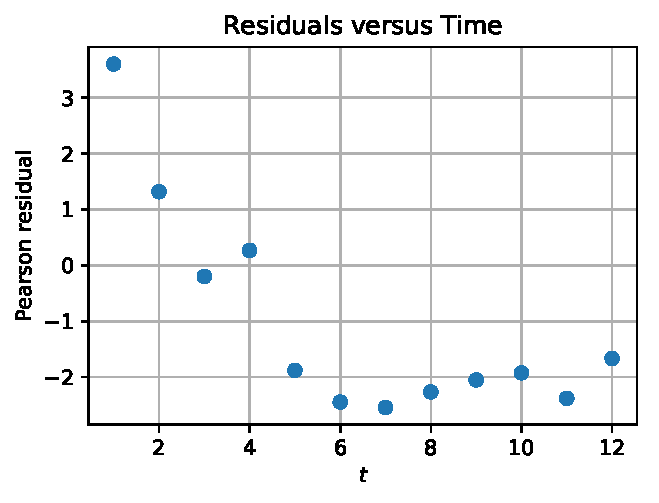
\includegraphics{p3_residuals.pdf}
        \caption{Residuals as a function of time with the MLE estimate.}
        \label{fig:p3_residuals}
      \end{figure}

      \begin{figure}
        \centering
        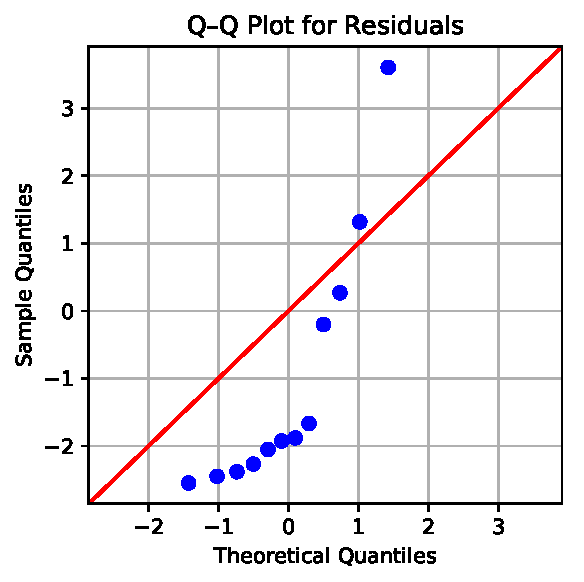
\includegraphics{p3_qq.pdf}
        \caption{Q--Q plot of residuals for the binomial model.}
        \label{fig:p3_qq}
      \end{figure}
            
      \begin{description}        
      \item[Solution:] Define $n_t = n - \sum_{s=1}^{t-1} Y_s$. The Pearson
        residuals are
        \begin{equation}
          \epsilon_t^\star = \frac{Y_t - n_t\hat{p}}
          {\sqrt{n_t\hat{p}\left(1 - \hat{p}\right)}}
          \label{eqn:p3_pearson_residual}          
        \end{equation}
        for $t = 1,2,\ldots,N$.

        The residuals are plotted in Figure \ref{fig:p3_residuals}. Clearly,
        there are not independent with respect to time. For earlier time steps,
        the probability of failure is underestimated, and for later time steps,
        the probability of failure is overestimated. Thus, component failure may
        not be a memoryless processe as assumed by our model.

        The Q--Q plot in Figure \ref{fig:p3_qq} indicates that the sample
        residuals are overdispersed relative to the theoretical quantiles. Since
        only the asymptotic behavior is normal, given only 12 observations, we
        might expect some deviation from normality, but qualitatively, the
        deviation is quite significant.
      \end{description}
    \item Fit a binomial model you feel is appropriate.
      \begin{table}
        \centering
        \begin{tabular}{lrrrr}
\toprule
{} &       MLE &  Standard error &  95\% CI lower bound &  95\% CI upper bound \\
\midrule
$\hat\beta_0$ & -0.090505 &        0.091144 &            -0.269143 &             0.088133 \\
$\hat\beta_1$ & -0.174740 &        0.026138 &            -0.225969 &            -0.123511 \\
\bottomrule
\end{tabular}

        \caption{MLE estimates for the model in Equation
          \ref{eqn:p3_binomial_model}.}
        \label{tab:p3_model_summary}
      \end{table}
      
      \begin{description}
      \item[Solution:] From Figure \ref{fig:p3_residuals}, there seems to be
        some sort of time dependence on the failure probability. That is, the
        probability of failure is not memoryless. Intuitively, one might
        hypothesize the longer that a component has surivived, the more robust
        it is, so the probability of failure should decrease with time.

        To test this hypothesis, we might fit the model:
        \begin{align}
          Y_t \mid Y_1,Y_2,\ldots, Y_{t-1}
          &\sim \operatorname{Binomial}\left(n_t, p_t\right)
          \label{eqn:p3_binomial_model} \\
          \operatorname{logit}\left(p_t\right)
          &= \beta_0 + \beta_1t. \nonumber
        \end{align}

        The score function for such a model would be obtained by replacing $p$
        with $p_t$ in Equation \ref{eqn:p3_likelihood}, taking the $\log$, and
        deriving with respect to $\beta = \begin{pmatrix} \beta_0 & \beta_1
        \end{pmatrix}^\intercal$.
        \begin{equation}
          S\left(\beta\right)
          = \sum_{t = 1}^N \left(
            Y_t - n_tp_t
          \right)
          \begin{pmatrix}
            1 \\
            t
          \end{pmatrix}.
          \label{eqn:p3_score}          
        \end{equation}

        The observed information is then
        \begin{equation}
          J\left(\beta\right)
          = \sum_{t=1}^N n_tp_t\left(1 - p_t\right)
          \begin{pmatrix}
            1 & t \\
            t & t^2
          \end{pmatrix}.
          \label{eqn:p3_observed_information}
        \end{equation}

        Using Equations \ref{eqn:p3_score}
        and \label{eqn:p3_observed_information}, we obtain MLE estimates and
        confidence intervals in Table \ref{tab:p3_model_summary}. The 95\%
        confidence interval for $\beta_1$ does not contain time, so we could
        reject a null hypothesis $\beta_1 = 0$ in test with significance level
        $0.05$. So, there is likely some correlation between time and failure
        probability.

        Figures \ref{fig:p3_residuals_time} and \ref{fig:p3_qq_time} indicate
        that our new model is much more appropriate. In Figure
        \ref{fig:p3_residuals_time}, there's no longer any obvious relationship
        between time and the residuals. In Figure \ref{fig:p3_qq_time}, we see
        the distribution of the residuals is quite close to normal.
      \end{description}

      \begin{figure}
        \centering
        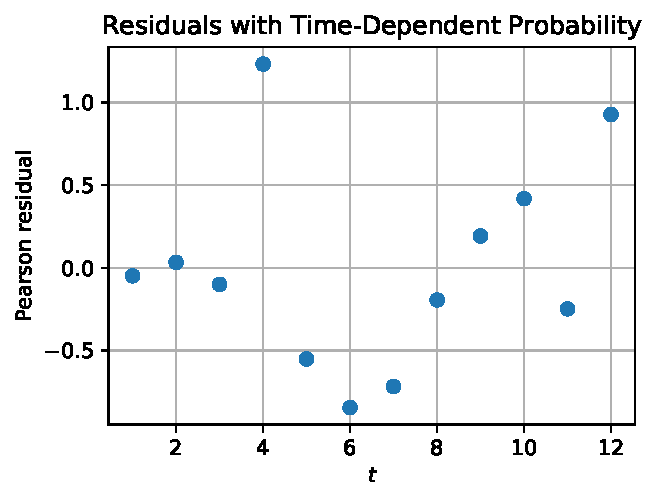
\includegraphics{p3_residuals_time.pdf}
        \caption{Residuals for the model in Equation \ref{eqn:p3_binomial_model}
          that lets the probability depend on time.}
        \label{fig:p3_residuals_time}
      \end{figure}

      \begin{figure}
        \centering
        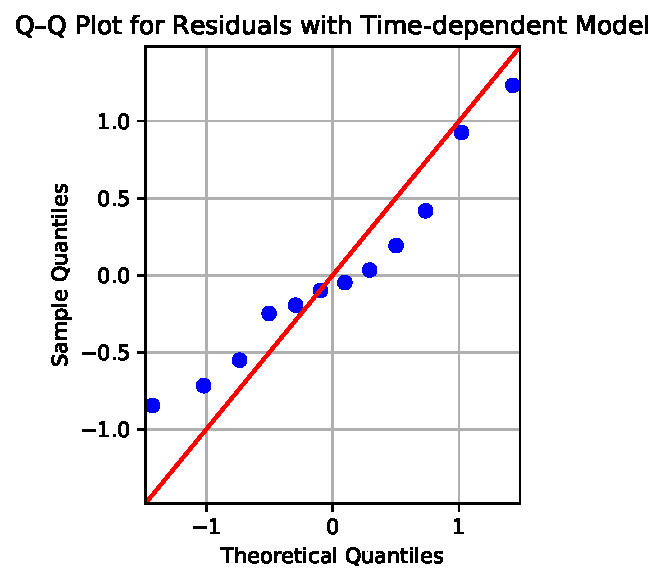
\includegraphics{p3_qq_time.pdf}
        \caption{Q--Q plot for the residuals plotted in Figure
          \ref{fig:p3_residuals_time}.}
        \label{fig:p3_qq_time}
      \end{figure}
    \end{enumerate}

    Code for histograms and model fitting can be found in
    \href{http://nbviewer.jupyter.org/github/ppham27/stat570/blob/master/final/failure\_time.ipynb}{\texttt{failure\_time.ipynb}}.
  \end{enumerate}

\begin{table}
  \centering
  \begin{tabular}{lrr}
\toprule
Time (weeks), $i$ &  Failures, $y_i$ &  Temperature, $x_i$ \\
\midrule
              $1$ &              210 &                24.0 \\
              $2$ &              108 &                26.0 \\
              $3$ &               58 &                24.0 \\
              $4$ &               40 &                26.0 \\
              $5$ &               17 &                25.0 \\
              $6$ &               10 &                22.0 \\
              $7$ &                7 &                23.0 \\
              $8$ &                6 &                20.0 \\
              $9$ &                5 &                21.0 \\
             $10$ &                4 &                18.0 \\
             $11$ &                2 &                17.0 \\
             $12$ &                3 &                20.0 \\
            $>12$ &               15 &                     \\
\bottomrule
\end{tabular}

  \caption{Time until failure for $n = 485$ components, along with average weekly
    temperature.}
  \label{tab:failure_time_data}
\end{table}
\end{document}
